\documentclass{article}
\usepackage{geometry}
\geometry{a4paper, right=2cm, left=2cm}
\usepackage{hyperref}
\usepackage{amsmath}
\usepackage{amssymb}
\usepackage{tikz}
\begin{document}
\title{Second Session of English for Computing}
\date{}
\maketitle
\tableofcontents
\section{Answer of the 12 Marbles Riddle} \label{sec:riddle}
Okay, let's wrap up the problem one more time. There are twelve marbles, $x_1, \ldots, x_{12}$, that are identical in shape (Figure~\ref{fig:init}). One them, weighs differently. We call it the divergent, outlier, or the fake one. We don't know if the divergent is \emph{heavier} or \emph{lighter} than the rest of the 11 marbles. We have a ballance scale that can tell the difference between the divergent and a normal marble. How to find the divergent with using the scale no more than three times?

\subsection{Answer}

\noindent At the beginning, \emph{all} of the marbles can potentially be the divergent. So we got 12 \emph{candidates} at the beginning. We denote candidates by $x$ and there will be $x_1, \ldots, x_{12}$ initially.
\begin{figure}
\center
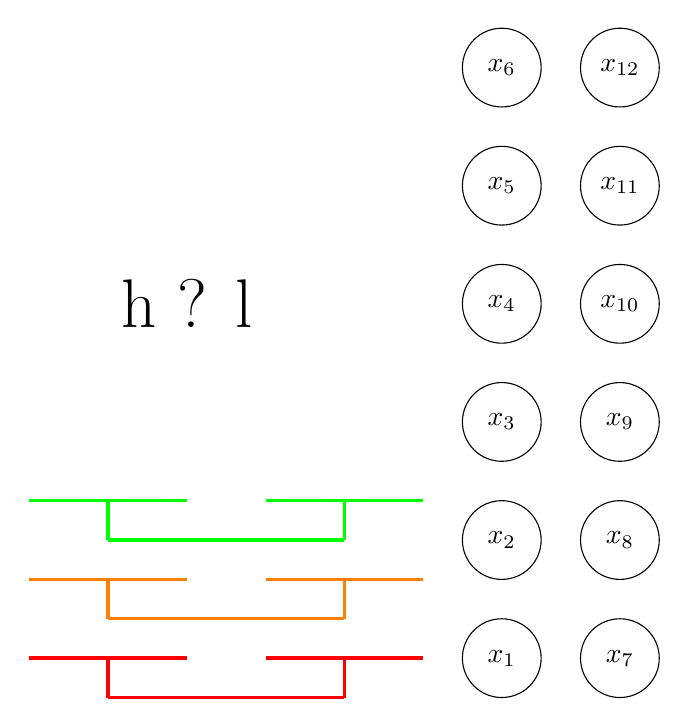
\begin{tikzpicture}
% \draw[step=1cm, gray, very thin] (0,0) grid (8,8);
% \foreach \x in {0,1,2,3,4,5,6,8}
% 	\draw (\x cm, 1pt) -- (\x cm, -1pt) node [anchor=north] {$\x$};
% \foreach \y in {1,2,3,4,5,6,7,8}
% 	\draw (1pt, \y cm) -- (-1pt, \y cm) node[anchor=east] {$\y$};
% drawing the scale
\draw[very thick, red] (0,0.5) -- (2,0.5);
\draw[very thick, red] (1,0.5) -- (1,0);
\draw[very thick, red] (1,0) -- (4,0);
\draw[very thick, red] (4,0) -- (4,0.5);
\draw[very thick, red] (3,0.5) -- (5,0.5);
% end of scale
% drawing the scale
\draw[very thick, orange] (0,1.5) -- (2,1.5);
\draw[very thick, orange] (1,1.5) -- (1,1);
\draw[very thick, orange] (1,1) -- (4,1);
\draw[very thick, orange] (4,1) -- (4,1.5);
\draw[very thick, orange] (3,1.5) -- (5,1.5);
% end of scale% drawing the scale
\draw[very thick, green] (0,2.5) -- (2,2.5);
\draw[very thick, green] (1,2.5) -- (1,2);
\draw[very thick, green] (1,2) -- (4,2);
\draw[very thick, green] (4,2) -- (4,2.5);
\draw[very thick, green] (3,2.5) -- (5,2.5);
% end of scale
% six circles
\draw (6,0.5) circle (0.5) node {$x_1$};
\draw (6,2) circle (0.5) node {$x_2$};
\draw (6,3.5) circle (0.5) node {$x_3$};
\draw (6,5) circle (0.5) node {$x_4$};
\draw (6,6.5) circle (0.5) node {$x_5$};
\draw (6,8) circle (0.5) node {$x_6$};
% six circles
\draw (7.5,0.5) circle (0.5) node {$x_7$};
\draw (7.5,2) circle (0.5) node {$x_8$};
\draw (7.5,3.5) circle (0.5) node {$x_9$};
\draw (7.5,5) circle (0.5) node {$x_{10}$};
\draw (7.5,6.5) circle (0.5) node {$x_{11}$};
\draw (7.5,8) circle (0.5) node {$x_{12}$};
%
	\node at (2, 5) {\Huge h ? l};
\end{tikzpicture}
	\caption{Initial setting.}
	\label{fig:init}
\end{figure}


We put $x_1, x_2, x_3$, and $x_4$ in one bucket, $x_5, x_6, x_7$, and $x_8$ in the other one. $x_9, x_{10}, x_{11}$, and $x_{12}$ are left outside (Figure~\ref{fig:t1}). The cases listed in table~\ref{tbl:try_1} are possible.
\begin{figure} % t1
\center
	\fbox{
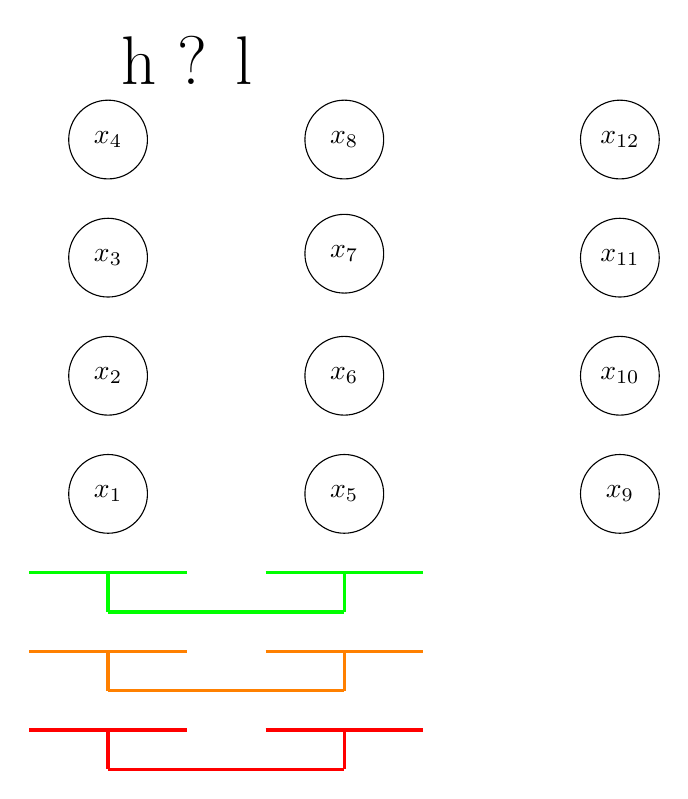
\begin{tikzpicture}
% \draw[step=1cm, gray, very thin] (0,0) grid (8,8);
% \foreach \x in {0,1,2,3,4,5,6,8}
% 	\draw (\x cm, 1pt) -- (\x cm, -1pt) node [anchor=north] {$\x$};
% \foreach \y in {1,2,3,4,5,6,7,8}
% 	\draw (1pt, \y cm) -- (-1pt, \y cm) node[anchor=east] {$\y$};
% drawing the scale
\draw[very thick, red] (0,0.5) -- (2,0.5);
\draw[very thick, red] (1,0.5) -- (1,0);
\draw[very thick, red] (1,0) -- (4,0);
\draw[very thick, red] (4,0) -- (4,0.5);
\draw[very thick, red] (3,0.5) -- (5,0.5);
% end of scale
% drawing the scale
\draw[very thick, orange] (0,1.5) -- (2,1.5);
\draw[very thick, orange] (1,1.5) -- (1,1);
\draw[very thick, orange] (1,1) -- (4,1);
\draw[very thick, orange] (4,1) -- (4,1.5);
\draw[very thick, orange] (3,1.5) -- (5,1.5);
% end of scale% drawing the scale
\draw[very thick, green] (0,2.5) -- (2,2.5);
\draw[very thick, green] (1,2.5) -- (1,2);
\draw[very thick, green] (1,2) -- (4,2);
\draw[very thick, green] (4,2) -- (4,2.5);
\draw[very thick, green] (3,2.5) -- (5,2.5);

% six circles
\draw (1, 3.5) circle (0.5) node {$x_1$};
\draw (1, 5) circle (0.5) node {$x_2$};
\draw (1, 6.5) circle (0.5) node {$x_3$};
\draw (1, 8) circle (0.5) node {$x_4$};
	\draw (4, 3.5) circle (0.5) node {$x_5$};
\draw (4, 5) circle (0.5) node {$x_6$};
\draw (4, 6.55) circle (0.5) node {$x_7$};
\draw (4, 8) circle (0.5) node {$x_8$};
\draw (7.5,3.5) circle (0.5) node {$x_9$};
\draw (7.5,5) circle (0.5) node {$x_{10}$};
\draw (7.5,6.5) circle (0.5) node {$x_{11}$};
\draw (7.5,8) circle (0.5) node {$x_{12}$};
%
	\node at (2, 9) {\Huge h ? l};
\end{tikzpicture}
}
	\caption{Our first try (with tag t1)}
	\label{fig:t1}
\end{figure} % t1
\begin{table} %t1.cs
	\caption{The possible states after the first weight}
	\label{tbl:try_1}
\begin{tabular}{|p{3cm}|p{5cm}|p{7cm}|}
	\hline
	Case tag& Case& Notation\\
	\hline
	\hline
	case t1.c1 (try 1, case 1)& $(x_1, x_2, x_3, x_4)>(x_5, x_6, x_7, x_8)$& We will have four marbles that have weighed heavier than the marbles in the other bucket. We denote them with $h$s (for \underline{h}eavier) and $l$s (for \underline{l}ighter): $h_1, h_2, h_3, h_4$ and $l_5, l_6, l_7, l_8$. Since these 8 marbles didn't balance, the divergent lies between them and the other 4 marbles that are left outside (i.e. $x_9, x_{10}, x_{11}$, and $x_{12}$) are normal marbles. We will denote them by $o$. So if case 1 happens, we will have $h, h, h, h, l, l, l, l, o, o, o, o$. Keep in mind that $h$s and $l$s are also candidates, while we know that $o$s are not candidates any more.\\
	\hline
	case t1.c2& $(x_1, x_2, x_3, x_4)=(x_5, x_6, x_7, x_8)$& Well, this means that the divergent lies within $x_9, x_{10}, x_{11}$, and $x_{12}$. So the state of the marbles will be: $x_9, x_{10}, x_{11}, x_{12}, o, o, o, o, o, o, o, o$.\\
	\hline
	case t1.c3& $(x_1, x_2, x_3, x_4)<(x_5, x_6, x_7, x_8)$& This is the exact opposite of case 1. It will probably be clear after we go through case 1, but if it isn't, I'll explain it for you.\\
	\hline
\end{tabular}
\end{table} % t1.cs

Let's first go through the second case (t1.c2). In this case, we have 4 candidates, 8 normals, two times to use the scale, and don't know if the divergent is heavier or lighter. In the second time, we put three of the candidates in one buckets and three normals in the other (Figure~\ref{fig:t1c2t2}). Again, three cases are possible that are listed in table~\ref{tbl:t1c2t2cs}.
\begin{figure} %t1.c2.t2
\center
	\fbox{
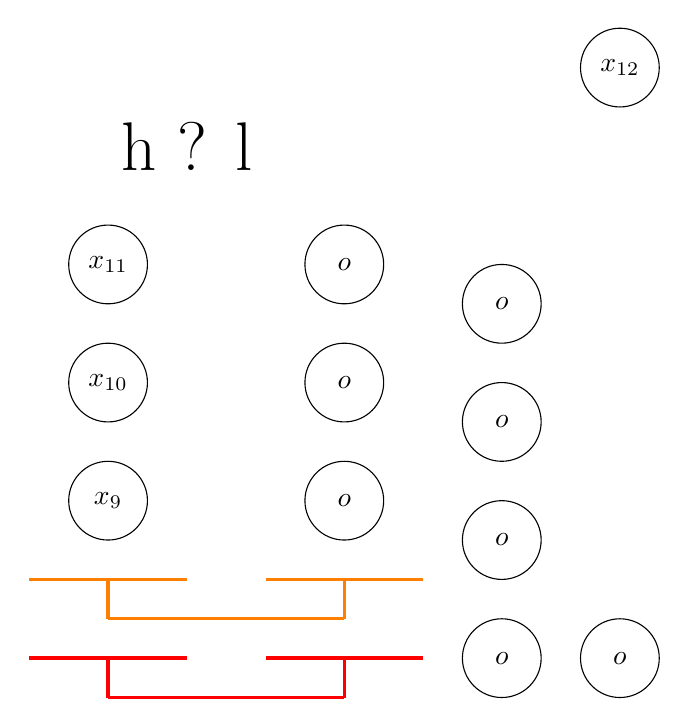
\begin{tikzpicture}
% \draw[step=1cm, gray, very thin] (0,0) grid (8,8);
% \foreach \x in {0,1,2,3,4,5,6,8}
% 	\draw (\x cm, 1pt) -- (\x cm, -1pt) node [anchor=north] {$\x$};
% \foreach \y in {1,2,3,4,5,6,7,8}
% 	\draw (1pt, \y cm) -- (-1pt, \y cm) node[anchor=east] {$\y$};
% drawing the scale
\draw[very thick, red] (0,0.5) -- (2,0.5);
\draw[very thick, red] (1,0.5) -- (1,0);
\draw[very thick, red] (1,0) -- (4,0);
\draw[very thick, red] (4,0) -- (4,0.5);
\draw[very thick, red] (3,0.5) -- (5,0.5);
% end of scale
% drawing the scale
\draw[very thick, orange] (0,1.5) -- (2,1.5);
\draw[very thick, orange] (1,1.5) -- (1,1);
\draw[very thick, orange] (1,1) -- (4,1);
\draw[very thick, orange] (4,1) -- (4,1.5);
\draw[very thick, orange] (3,1.5) -- (5,1.5);
% end of scale% drawing the scale
% six circles
\draw (6,0.5) circle (0.5) node {$o$};
\draw (6,2) circle (0.5) node {$o$};
\draw (6,3.5) circle (0.5) node {$o$};
\draw (6,5) circle (0.5) node {$o$};
\draw (4,5.5) circle (0.5) node {$o$};
\draw (4,4) circle (0.5) node {$o$};
% six circles
\draw (7.5,0.5) circle (0.5) node {$o$};
\draw (4, 2.5) circle (0.5) node {$o$};
\draw (1,2.5) circle (0.5) node {$x_9$};
\draw (1,4) circle (0.5) node {$x_{10}$};
\draw (1,5.5) circle (0.5) node {$x_{11}$};
\draw (7.5,8) circle (0.5) node {$x_{12}$};
%
	\node at (2, 7) {\Huge h ? l};
\end{tikzpicture}
}
	\caption{Try tag : t1.c2.t2 (second try, when case 2 happens, in our 1st try)}
	\label{fig:t1c2t2}
\end{figure} % t1c2t2
\begin{table} %t1c2t2cs
	\caption{Possible cases of t1c2t2}
	\label{tbl:t1c2t2cs}
\begin{tabular}{|p{3cm}|p{5cm}|p{7cm}|}
	\hline
	Case tag& Case& Notation\\
	\hline
	\hline
	 t1c2t2c1& $(x_9, x_{10}, x_{11})>(o, o, o)$& This means that the divergent lies between $x_9, x_{10}$, and $x_{11}$. It also tells us that the outlier is heavier. So we will have three candidates, 9 normals, another time to use the scale, and the knowledge about outlier's relative weight in comparison to the normals.\\
	\hline
	case t1c2t2c2&$(x_9, x_{10}, x_{11})=(o, o, o)$& Well, you're expected to deduce that the outlier is $x_{12}$ in this case.\\
	\hline
	case t1c2t2c3& $(x_9, x_{10}, x_{11})<(o, o, o)$& This is the exact opposite of t1c2t2c3. It will probably be clear after we go through t1c2t2c3, but if it isn't, I'll explain it for you.\\
	\hline
\end{tabular}
\end{table} % t1c2t2cs

In the case of t1c2t2c1, we're gonna use the scale for the last time. As mentioned in the table, this means that the outlier lies within $x_9, x_{10}$, and $x_{11}$ and we also know that it is heavier. We put $x_{9}$ on the left, and $x_{10}$ on the right. If they balanced, well, $x_{11}$ is the outlier. If they didn't, the heavier one is the outlier.

How about summing up what we have seen by far? 
\begin{enumerate}
	\item We devided the marbles into three groups of four
	\item Compared two of the groups.
	\item Took care of what will happen if they balanced (i.e. the case t1c2)
\end{enumerate}
What we should do now, is to see what to do if they do not balance (i.e. the case t1c1).
\subsubsection{The case t1c1}
In case t1c1, we fill the buckets for the second time, as in Figure~\ref{fig:t1c1t2}. Possible cases are discussed in table~\ref{tbl:t1c1t2cs}
\begin{figure} %t1c1t2
\center
	\fbox{
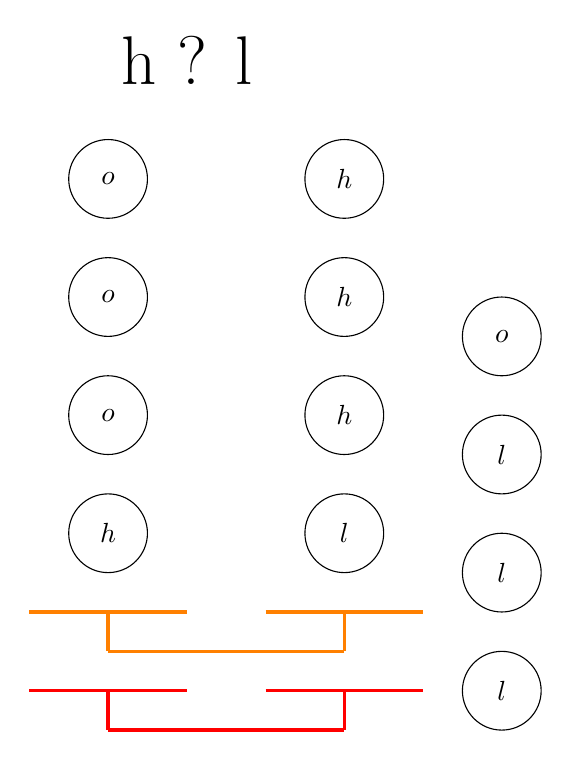
\begin{tikzpicture}
% \draw[step=1cm, gray, very thin] (0,0) grid (8,8);
% \foreach \x in {0,1,2,3,4,5,6,8}
% 	\draw (\x cm, 1pt) -- (\x cm, -1pt) node [anchor=north] {$\x$};
% \foreach \y in {1,2,3,4,5,6,7,8}
% 	\draw (1pt, \y cm) -- (-1pt, \y cm) node[anchor=east] {$\y$};
% drawing the scale
\draw[very thick, red] (0,0.5) -- (2,0.5);
\draw[very thick, red] (1,0.5) -- (1,0);
\draw[very thick, red] (1,0) -- (4,0);
\draw[very thick, red] (4,0) -- (4,0.5);
\draw[very thick, red] (3,0.5) -- (5,0.5);
% end of scale
% drawing the scale
\draw[very thick, orange] (0,1.5) -- (2,1.5);
\draw[very thick, orange] (1,1.5) -- (1,1);
\draw[very thick, orange] (1,1) -- (4,1);
\draw[very thick, orange] (4,1) -- (4,1.5);
\draw[very thick, orange] (3,1.5) -- (5,1.5);
% end of scale% drawing the scale
% six circles
\draw (6,0.5) circle (0.5) node {$l$};
\draw (6,2) circle (0.5) node {$l$};
\draw (6,3.5) circle (0.5) node {$l$};
\draw (6,5) circle (0.5) node {$o$};
\draw (4,7) circle (0.5) node {$h$};
\draw (4,5.5) circle (0.5) node {$h$};
% six circles
\draw (4, 4) circle (0.5) node {$h$};
\draw (4, 2.5) circle (0.5) node {$l$};
\draw (1,2.5) circle (0.5) node {$h$};
\draw (1,4) circle (0.5) node {$o$};
\draw (1,5.5) circle (0.5) node {$o$};
\draw (1,7) circle (0.5) node {$o$};
%
	\node at (2, 8.5) {\Huge h ? l};
\end{tikzpicture}
}
	\caption{t1c1t2}
	\label{fig:t1c1t2}
\end{figure} % t1c1t2
\begin{table} %t1c1t2cs
	\caption{Possible cases of t1c1t2}
	\label{tbl:t1c1t2cs}
\begin{tabular}{|p{3cm}|p{5cm}|p{7cm}|}
	\hline
	Case tag& Case& Notation\\
	\hline
	\hline
	 t1c1t2c1& $(o,o,o,h)>(h,h,h,l)$& In this case, either the $h$ on the left is the outlier, or the the $l$ on the right. (If don't understand why, here's an explanation. When the buckets do not balance, the outlier is definitely on the scale. It isn't among the three normals on the left of course; we already know that they are normal. The three $h$s on the right, are either normal, or a heavier outlier. If they contain the outlier and the outlier is lighter, they wouldn't have gone down in the 1st try (t1.c1). So we will be left with the heavy on the left and the light on the right. Text will explain how to handle this case.\\
	\hline
	case t1c1t2c2&$(o,o,o,h)=(h,h,h,l)$& So the outlier is not on the scale and we are only left with the three $l$s outside. We will have one more time to use the scale, and know the relative weight of the divergent in comparison to the normals. This is similar to the solution provided for t1c2t2c1. If you cannot figure it out, ask it. \\
	\hline
	case t1c1t2c3& $(o,o,o,h)<(h,h,h,l)$& It doesn't balance, so the outlier is on the scale. The left side is lighter and contains only one candidate, the $h$.( The other three are $o$s.) If the $h$ on the left is the outlier, it must be lighter, but this isn't possible, since it was among the heavies in t1c1. So we will be left with the four marbles on the right and we'll also conclude that the divergent is heavier. Long story short, it is among the three $h$s on the right, and the solution is similar to t1c2t2c1 and t1c1t2c2\\
	\hline
\end{tabular}
\end{table} % t1c2t2cs

We will explore t1c1t2c1. In summary:
\begin{itemize}
	\item We have two candidates and 10 normals.
	\item We have one more time to use the scale.
	\item We don't know the if the outlier is heavier or lighter.
\end{itemize}
It's easy. We place one of the candidates on the left and a normal on the right. If they balance, the divergent is the one that was left out. Otherwise, the divergent is the on the left bucket.
\subsection{Exercise}
\begin{enumerate}
	\item In these explanations, find the words, phrases, or statements, that you think you will encounter again as a computer scientist.
	\item Find usages for these handy language structures in other sources. (You may come up with authentic usages yourself.)
	\item Explain the answer in your languge. (delivered as a written answer)
	\item Do the above with the question (i.e. explain the 12-marbles-riddle's question).
\end{enumerate}
\section{A Sample Reading Test}
We took the reading test available at \href{https://ieltspracticeonline.com/ielts-reading-27-hard-disk-drive-technology/}{https://ieltspracticeonline.com/ielts-reading-27-hard-disk-drive-technology/}. It was about hard disk drives, a storage medium.
\subsection{Exercises}
\begin{enumerate}
	\item List the technical terminology that you think are probable to pop up again, when you're reading another computer-related text.
	\item Interested students can prepare a presentation, explaining how hard disk drives work, what are partitions, different formats, etc. 
\end{enumerate}
\end{document}
